% The one-node graph of the home page, with a self-loop for each of the two
% modes, in the mode colors of docs/graph_drawing.jl. Compile to SVG with
%   latex common_graph.tex && dvisvgm --no-fonts --bbox=papersize common_graph.dvi
\def\pgfsysdriver{pgfsys-dvisvgm.def}
\documentclass[tikz, border = 3pt]{standalone}
\usetikzlibrary{arrows.meta}
\definecolor{mode1}{HTML}{4169E1} % royalblue
\definecolor{mode2}{HTML}{FF8C00} % darkorange
\renewcommand{\familydefault}{\sfdefault}
\begin{document}
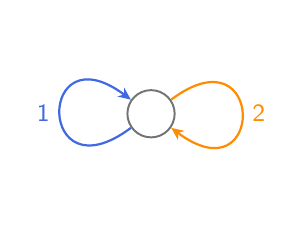
\begin{tikzpicture}[
    > = {Stealth[length = 1.6mm, width = 1.4mm]},
    self loop/.style = {->, line width = 0.8pt},
  ]
  \node[circle, draw = black!55, fill = white, line width = 0.7pt,
        minimum size = 6mm] (a) {};
  \draw[self loop, mode1] (a.215) .. controls +(-12mm, -9mm) and +(-12mm, 9mm)
    .. node[left] {\small 1} (a.145);
  \draw[self loop, mode2] (a.35) .. controls +(12mm, 9mm) and +(12mm, -9mm)
    .. node[right] {\small 2} (a.-35);
\end{tikzpicture}
\end{document}
